
%==============================================
\section{Governing relations}
\label{sec:governing_eqs}
%==============================================

If not specified, the International System of Units (SI) is used in this document.
In particular, hats ``$\hat{...}$'' refer to quantities which are \emph{not} expressed in SI units. The following alternative units are employed: 
\begin{itemize}
    \item $\hat n$ is the density in $10^{19} \si{m^{-3}}$: 
    $\hat n = 10^{-19}\,n_{\si{[m^{-3}]}}$
    \item $\hat T$ is the temperature in $keV$: $\hat T = 10^{-3}\, k_B T_{[K]}\,/e$ \\(with $k_B \approx 1.3807\, 10^{-23} \si{J.K^{-1}}$ the Boltzmann's constant and $e\approx 1.6022\, 10^{-19}C$ the elementary electric charge)
    \item $\hat I_p$ is the plasma current in MA: $\hat I_p = 10^{-6}\,I_{p\,[A]}$
    \item $\hat P$ is the power in MW: $\hat P = 10^{-6}\, P_{[W]}$
    \item $\hat M$ is the mass in Atomic Mass Unit
\end{itemize}

%----------------------------------------------
\subsection{Geometry}

We recall that the volume of a tore can be approximated\footnote{The expression is exact for $\kappa=1$.} by 
\begin{equation}
V_t = 2\pi^2 \kappa R a^2
\end{equation}
with $a$ the minor radius and $R$ the major radius of the tore. Here, $\kappa=b/a$ stands for the elongation of the plasma, $b$ being the largest radius of the ellipsoid. $\kappa=1$ for a circular cross-section, and is larger than unity for an elongated plasma.
Introducing the inverse aspect ratio $\varepsilon$ defined as $\varepsilon  \doteq a /R$, the volume then reads:
\begin{equation}
\boxed{V_t = 2\pi^2 \kappa \varepsilon^2 R^3}
\label{eqn:tore_volume}
\end{equation}

%----------------------------------------------
\subsection{Plasma current}
Integrating the Maxwell-Amp\`ere equation over the whole plasma cross-section, and using Stokes' theorem, one gets:
\begin{equation}
\int_\mathcal{S} (\nablabf\times \Bbf) \cdot \mathbf{dS} = 
\oint_\mathcal{C} \mathbf{B} \cdot \mathbf{d\ell}
= \mu_0 \int_\mathcal{S} \jbf \cdot \mathbf{dS} = \mu_0 I_p
\end{equation}
Neglecting the elongation of the cross-section, the equation can be approximated as follows
$$
2\pi a B_p = \mu_0 I_p
$$
with $B_p$ the poloidal component of the magnetic field at the separatrix. In the limit of large aspect ratios, it can be easily related to the safety factor $q_a$ at the separatrix\footnote{Actually, $q_a$ is usually taken slightly inside the separatrix, at 95$\%$ of the poloidal magnetic flux.}:
\begin{equation}
q_a \doteq \frac{a}{R} \frac{B_t}{B_p} 
\end{equation}
with $B_t$ the toroidal component of the magnetic field at the magnetic axis. Then it comes:
\begin{equation}
\boxed{\hat I_p = C_I \frac{\varepsilon^2}{q_a} \; R B}
\label{eqn:plasma_current}
\end{equation}
where $\hat I_p$ is the current expressed in MA, and $C_I = 2\pi\, 10^{-6} /\mu_0 = 5$  ($\mu_0 = 4\pi\, 10^{-7} \si{H.m^{-1}}$).
Notice that $B_t$ has been safely replaced by $B$ since $B_p\ll B_t$ in tokamak plasmas. 

%----------------------------------------------
\subsection{Greenwald density}

As stated in a recent topical review on the subject \cite{Greenwald2002}, \emph{``in addition to the operational limits imposed by MHD stability on plasma current and pressure, an independent limit on plasma density is observed in confined toroidal plasmas. [...] In tokamaks, [...] there is strong evidence linking the limit to physics near the plasma boundary [...]''}. As a matter of fact, the so-called Greenwald density $n_G$ is not a sharp density limit, since discharges with peaked density profiles can well operate above this value. So far, there is no widely accepted, first principles model for the density limit. Yet, the focus is currently either on mechanisms which lead to strong edge cooling, or on collisionality enhanced turbulent transport.

From \cite[eq.(14.146)]{Freidberg2007}, the most common empirical scaling for (line-averaged) density limit is the following:
\begin{equation}
\boxed{\hat n_G \doteq C_n \frac{\hat I_p}{\varepsilon^2 R^2}  }
\label{eqn:greenwald_density}
\end{equation}
with $C_n = 10/\pi \approx 3.18$.
Using the expression of the plasma current given above, and replacing $\mu_0$ by its value, $\hat n_G$ can be recast as follows:
\begin{equation}
\hat n_G = C_nC_I \frac{B}{q_aR}
\end{equation}
Finally, one introduces the normalised density $n_N\doteq n/ n_G$, so that:
\begin{equation}
  \hat n = C_nC_I\; n_N\; \frac{B}{q_aR}
  \label{eq:n_nN}
\end{equation}

%----------------------------------------------
\subsection{Plasma beta}
The plasma beta $\beta$ is defined as the ratio of the plasma pressure $p=2nk_BT$ (the factor 2 comes from the fact that the total temperature is considered, $i.e.$ $n(T_e+T_i)$, with the assumption of equal ion and electron temperatures) to the magnetic pressure $B^2/2\mu_0$:
\begin{equation}
\boxed{\beta_\% \doteq \frac{p}{B^2/2\mu_0}
 = C_\beta \frac{\hat n \hat T}{B^2}}
\label{eqn:beta}
\end{equation}
where $\beta_\%=10^2\, \beta$ is expressed in $\%$ and $C_\beta = 4.\,10^2\mu_0\times 10^{19}\times 10^3 e \approx 0.805$.

Several modes (such as e.g. kink, tearing or ballooning modes) become MHD unstable above certain thresholds of pressure gradient and plasma current, so that one can expect that $\beta$ will be subject to a stability limitation which will likely depend on the plasma current. \emph{``However, the concept of $\beta$ limit is not precise. Stability depends on profiles, and any optimisation introduces the questions of which modes of instability to include and what mode numbers to allow. Furthermore, there is uncertainty as to the severity of the nonlinear consequences of the various modes. Nevertheless the intrinsic usefulness of a concise analytic $\beta$ limit in assessing possible tokamak performance has prompted a number of investigations''} \cite{Wesson2004}.

It turns out that the $\beta$ limit, i.e. the maximum stable $\beta$, scales approximately like $\varepsilon/q_a$, which can be recast as $(\mu_0/2\pi)\; I_p/aB$ from the above relations. We shall define $\beta_m$ as follows:
\begin{equation}
  \beta \leqslant \beta_m \doteq g\; \frac{\hat I_p}{a B}
\end{equation}
The coefficient of proportionality $g$ depends on the considered instabilities. The so-called "Troyon limit" \cite{Troyon1984} puts this coefficient to $2.8\, 10^{-2}$ (or 2.8 if $\beta$ is expressed in $\%$).
It is usual to introduce the normalised $\beta$, called $\beta_N$, defined by \cite[eq.(13.146)]{Freidberg2007}:
\begin{equation}
    \beta \doteq \beta_N \frac{\hat I_p}{a B}
\end{equation}
Then, the stability limit simply reads $\beta_N <g$.

Interestingly, using the above expression and that of the plasma current (\ref{eqn:plasma_current}), the plasma pressure can be expressed as a function of $\beta_N$ and $B$:
\begin{eqnarray}
  \hat n\hat T &=& C_\beta^{-1} \beta_N \frac{\hat I_p B}{\varepsilon R} \nonumber \\
    &=& \frac{C_I}{C_\beta}\; \frac{\varepsilon}{q_a} \;  \beta_N B^2
  \label{eqn:nT_betaN}
\end{eqnarray}

%----------------------------------------------
\subsection{Fusion power}

To get nuclear fusion, nuclei have to come close enough to each other. Nuclear forces can overcome their mutual electrostatic repulsion provided their distance becomes of the order of 1 Fermi ($10^{-15}$m). This would require temperatures of the order of 720 keV for head-on collisions of thermal particles to lead to fusion reactions in a classical way. Actually, quantum physics has to be taken into account in the process. Both in tokamaks and in stars interiors, fusion reactions take place predominantly due to the tunnel effect. Crossing this barrier can be quantified in a probabilistic manner with the reaction rate $R$ $[\mathrm{reaction/m^3 s}]$, defined as the probability of reaction per unit time and volume. The reaction rate between mono-energetic ions of density $n_1$ $\mathrm{[m^{-3}]}$ striking target ions of density $n_2$ $\mathrm{[m^{-3}]}$ is proportional to the effective cross-section area $\sigma$ $\mathrm{[m^2]}$ and to the velocity difference $v_{12}$ between the two species:
\begin{equation}
r_{12} = n_1 n_2 \; \sigma v_{12}
\end{equation}
The quantity  $\sigma v_{12}$, which depends on the kinetic energy of the colliding particles, is called the reactivity ($\mathrm{[m^3/s]}$). Note that the reaction rate $r_{12}$ is proportional to the square of the density of the mixture. In fusion plasmas, ions are not mono-energetic. They are assumed to have Maxwellian velocity distributions. The average reactivity $\langle \sigma v \rangle_{12}$ derives from the following expression:
\begin{equation}
\left < \sigma v \right >_{12} 
= \int_{-\infty}^{+\infty} \int_{-\infty}^{+\infty} 
\sigma(v_{12}) v_{12}\;  f_1(v_1) f_2(v_2) \; dv_1dv_2
\end{equation}
Finally, the average reaction rate $R_{12}$ reads:
\begin{equation}
R_{12} = n_1 n_2 \; \left < \sigma v \right >_{12}
\end{equation}
It governs the time evolution of both densities: $dn_1/dt = dn_2/dt = -R_{12}$.
The temperature dependence of the reactivity $\langle \sigma v \rangle_{12}$ is plotted on figure \ref{fig:reactivity} for several fusion reactions (data from \cite{Huba2013}).

\begin{figure} 
\begin{center}
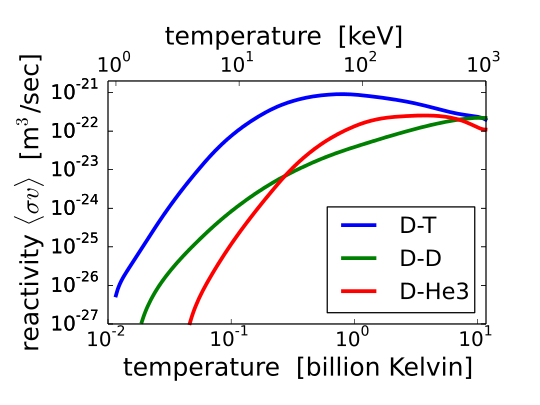
\includegraphics[width=0.75\textwidth]{figures/reactivity_DT.png}
\caption{Fusion reactivity }
\label{fig:reactivity}
\end{center}
\end{figure}

The D-T reactivity reaches its maximum for a temperature of 64 keV, corresponding to a temperature of $742\,10^6$ K. Since it has the highest reaction rate, the D-T reaction is the “easiest” to initiate (maximum reactivity at lowest temperature) of all fusion reactions and is the targeted fusion reaction\cite{FusionCEA1987}: 
\begin{equation}
\mathrm{D + T} \longrightarrow \mathrm{{}^4 He~(3.56~MeV) + n~(14.03~MeV)}
\end{equation}
The D-T reaction leads to a total released energy of $E_{DT}$ = 17.59 \si{MeV} = $2.82\times 10^{-12} \si{J}$ per fusion reaction\footnote{This value can be compared to the 200 MeV released by $^{235}$U fission. Yet, the energy release \emph{per nucleon} ($i.e.$ per kilogram) is approximately 4 times larger for fusion than for fission reactions.}. Notice that the ratio of the total energy to that carried by the alpha particles $\lambda \doteq 17.59/3.56 \approx 4.94$ is not exactly equal to 5 as one would expect on the basis of momentum conservation. Actually, this ratio \emph{is obviously} consistent with momentum conservation, as it should, provided one takes into account relativistic effects. This point is detailed in appendix \ref{appendix:fusion_power}.

The fusion power per unit volume $p_{DT}$ produced by the fusion of the nuclei of deuterium and tritium reads: 
\begin{equation}
  p_{DT} = n_D n_T \left< \sigma v \right>_{DT} E_{DT}
\end{equation}
with $n_D$ and $n_T$ the deuterium and tritium density and $\left< \sigma v \right>_{DT}$ the D-T reactivity. Assuming equal deuterium and tritium densities:
\begin{equation}
  n_D = n_T = \frac{n}{2}
\end{equation}
with $n$ the electron density, then the thermonuclear power density is:
\begin{equation}
  p_{DT} = \frac{1}{4} n^2 \left< \sigma v \right>_{DT} E_{DT}
\end{equation}

Assuming a constant reactivity in the plasma (``flat profile hypothesis'') and using the tore volume \ref{eqn:tore_volume}, the fusion power then reads:
\begin{equation}
  P_{DT} = \frac{\pi^2 \kappa \varepsilon^2}{2} 
  R^3 n^2 \left< \sigma v \right>_{DT} E_{DT}
\end{equation}
In the temperature range 10.3-18.5 keV, it turns out that the reactivity $\left< \sigma v \right>_{DT}$ can well (with about 10$\%$ error) be approximated by\cite[(1.5.4)]{Wesson2004}: 
\begin{equation}
  \left< \sigma v \right>_{DT} \approx 1.18\, 10^{-24}\; \hat T^2 \;\si{\left[m^3 s^{-1}\right]}
\end{equation}
All in all, one gets (in MW):
\begin{equation}
  \hat P_{DT} = C_{fus} \kappa \varepsilon^2 R^3 \hat n^2 \hat T^2  
\label{eq:DT_fusion_power}
\end{equation}
with $C_{fus} \approx 17.59 \times e\times 1.18\, 10^{-24} \times 10^{2\times19}\times \pi^2/2 \approx 1.64\, 10^{-3}$. We recall here that $\hat T$ is expressed in keV, and $\hat n$ in $10^{19} \, \si{m^{-3}}$. 
Notice that the fusion power can also be expressed in terms of $\beta_N$by using eq.\ref{eqn:nT_betaN}:
\begin{equation}
  \hat P_{DT} = \frac{C_{fus}C_I^2}{C_\beta^2} \frac{\kappa \varepsilon^4}{q_a^2} 
    \beta_N^2 R^3 B^4 
\label{eq:DT_fusion_power_betaN}
\end{equation}
This total fusion power is distributed among the alpha particles and the neutrons: 
\begin{equation}
  P_{DT} = P_\alpha + P_n = \lambda \; P_\alpha
\end{equation}
where we recall that $\lambda \approx 4.94$. Due to the mass ratio, almost 80\% of the power is carried by the neutrons. 

%----------------------------------------------
\subsection{Plasma heating and amplification factor Q}

Conversely to neutrons which leave the plasma, charged $\alpha$ nuclei are confined by the magnetic field and should ideally transfer their energy to the main ions before being extracted\footnote{There are basically 2 ways for this energy transfer. Since the collision frequency scales like the velocity difference between the colliding species to the power $-3$ ($\nu_{coll,ss'}\sim n_{s'}/\Delta v_{ss'}^3$), alpha particles transfer their energy dominantly to the electrons, which are much faster due to their low inertia. Then two routes are possible for the energy transfer from the electrons to the ions. Either via collisions, or via turbulence. In the latter case, the mediator are the electrostatic plasma waves. The relative weight of those two channels is still a matter of research.}. The total -- or net -- heating power is the sum of the auxiliary plasma heating -- including Ohmic heating -- and of alpha heating:
\begin{equation}
P_{net} \doteq P_\alpha + P_{ext}
\label{eq:net_power}
\end{equation}
The plasma amplification factor is defined as:
\begin{equation}
Q \doteq \frac{P_{DT}}{P_{ext}}
\label{eq:Q}
\end{equation}
Importantly, notice that $Q$ \emph{does not} encompass -- by far -- the entire question of the energetic efficiency of a fusion reactor. Indeed, in particular, it does neither account for the energy used for cryogenic purposes (as required by the use of superconductors) nor for the conversion factor of thermal to electric energy\footnote{This point is often misleading for the public and it is important to be factually correct. Misleading statements concerning fusion and ITER power and energy since decades have been highlighted in \url{http://news.newenergytimes.net/2017/10/06/the-iter-power-amplification-myth/}. This led directly ITER to update its public information web pages on the Q-factor (cf. \url{https://www.iter.org/newsline/-/2845}).  Cf. also the follow-up \url{http://news.newenergytimes.net/2017/12/11/evidence-of-the-iter-power-deception/}}.

The net power can therefore be expressed in terms of the fusion power and of the amplification factor:
\begin{equation}
\boxed{
P_{net} = P_{DT} \; \frac{1+Q/\lambda}{Q}
}
\label{eq:Pnet_PDT_Q}
\end{equation}
Replacing $P_{DT}$ by its expression eq.\ref{eq:DT_fusion_power}, one finally obtains:
\begin{equation}
  \hat P_{net} = C_{fus} \kappa \varepsilon^2 R^3 \hat n^2 \hat T^2 \; \frac{1+Q/\lambda}{Q}
\label{eq:Pnet_QnTR}
\end{equation}


%----------------------------------------------
\subsection{Power loss and energy confinement time}

The total internal energy of the plasma reads as follows:
\begin{equation}
  W  = \int \frac{3}{2} k_B \left( n_e T_e + n_i Ti \right ) dV 
  \approx \int 3 n k_BT dV
\end{equation}
where the integral is performed over the plasma volume. Here, equal ion and electron temperatures have been assumed. Assuming flat density and temperature profiles and using the expression of the volume of a torus eq.\ref{eqn:tore_volume}, the total plasma internal energy then reads (in [MW.s]):
\begin{equation}
  \hat W = C_{loss} \kappa \varepsilon^2  \hat n \hat T R^3
\label{eq:total_energy}
\end{equation}
where $C_{loss} = 6\pi^2 \times 10^{19} \times 10^{-3}e \approx 0.095$.

The energy confinement time $\tau_E$ is usually defined as the characteristic time at which this energy is lost from the plasma due to thermal transport\footnote{This definition excludes radiative losses. It is consistent with the one used for the ITER scaling laws, discussed in section \ref{sec:scaling_law}.}, either by collisional conduction or by turbulent thermal convection. It is defined as follows:
\begin{equation}
\boxed{
  \hat P_{loss} \doteq \frac{\hat W}{\tau_E} 
  = C_{loss} \kappa \varepsilon^2  \frac{\hat n \hat T R^3}{\tau_E}
}
\label{eq:Ploss}
\end{equation}
Similarly to what we did for the D-T fusion power, $P_{loss}$ can also be expressed as a function of $\beta_N$ (using eq.\ref{eqn:nT_betaN}):
\begin{equation}
  \hat P_{loss} = \frac{C_{loss}C_I}{C_\beta}  \frac{\kappa \varepsilon^3}{q_a}
    \frac{\beta_N R^3 B^2}{\tau_E}
\label{eq:Ploss_betaN}
\end{equation}


%----------------------------------------------
\subsection{The triple product and the Lawson criterion}
At equilibrium, the total heating power is equal to the loss power. Using the previous definitions, this translates into $P_{net} =P_{loss}$ \footnote{Should the plasma not be at equilibrium and/or be subject to significant radiative losses in the confined region, then $P_{net}$ should be replaced by $(P_{net}-dW/dt-P_{rad})$. The subtraction of $P_{rad}$ ensures the balance equation to be consistent with the retained definition of $\tau_E$.}.
Using both expressions of the powers, more precisely eq.\ref{eq:Pnet_QnTR} and eq.\ref{eq:Ploss}, one then obtains an expression for the so-called triple product $nT\tau_E$:
\begin{equation}
\boxed{
  \hat n \hat T \tau_E = \frac{C_{loss}}{C_{fus}} \frac{Q}{1+Q/\lambda} }
\label{eq:nTtau_Q}
\end{equation}

The Lawson criterion corresponds to the limit when $Q\to\infty$, $i.e.$ when the entire plasma heating is provided by alpha heating ($P_{net}=P_\alpha$). In this case, one gets:
\begin{equation}
  \hat n \hat T \tau_{E,L} \doteq \frac{\lambda C_{loss}}{C_{fus}}
\label{eq:nTtau_Lawson}
\end{equation}
With our present calculation, assuming flat density and temperature profiles, one finds $\lambda C_{loss}/C_{fus} \approx 286$, which is close to the more standard value of 300. This means that, for a plasma density of $\hat n=10$ (hence $n=10^{20}\si{m^{-3}}$) at the temperature of $\hat T=10$keV, the confinement time imposed by the Lawson criterion is of order of $\tau_{E,L} \approx 3s$.

It is instructive to consider how the amplification factor $Q$ varies with the energy confinement time normalised to the Lawson time, fig.\ref{fig:Q_tauE}. Combining eq.\ref{eq:nTtau_Q} and eq.\ref{eq:nTtau_Lawson}, one readily obtains:
\begin{equation}
    Q = \frac{\lambda}{\tau_{E,L}/\tau_E - 1}
\end{equation}
As expected, $Q$ diverges when $\tau_E = \tau_{E,L}$. Since $\lambda \approx 5$, one finds that $Q=5$ is reached for $\tau_E \approx \frac{1}{2}\; \tau_{E,L}$, and $Q=10$ for $\tau_E \approx \frac{2}{3}\; \tau_{E,L}$.

\begin{figure} 
	\begin{center}
		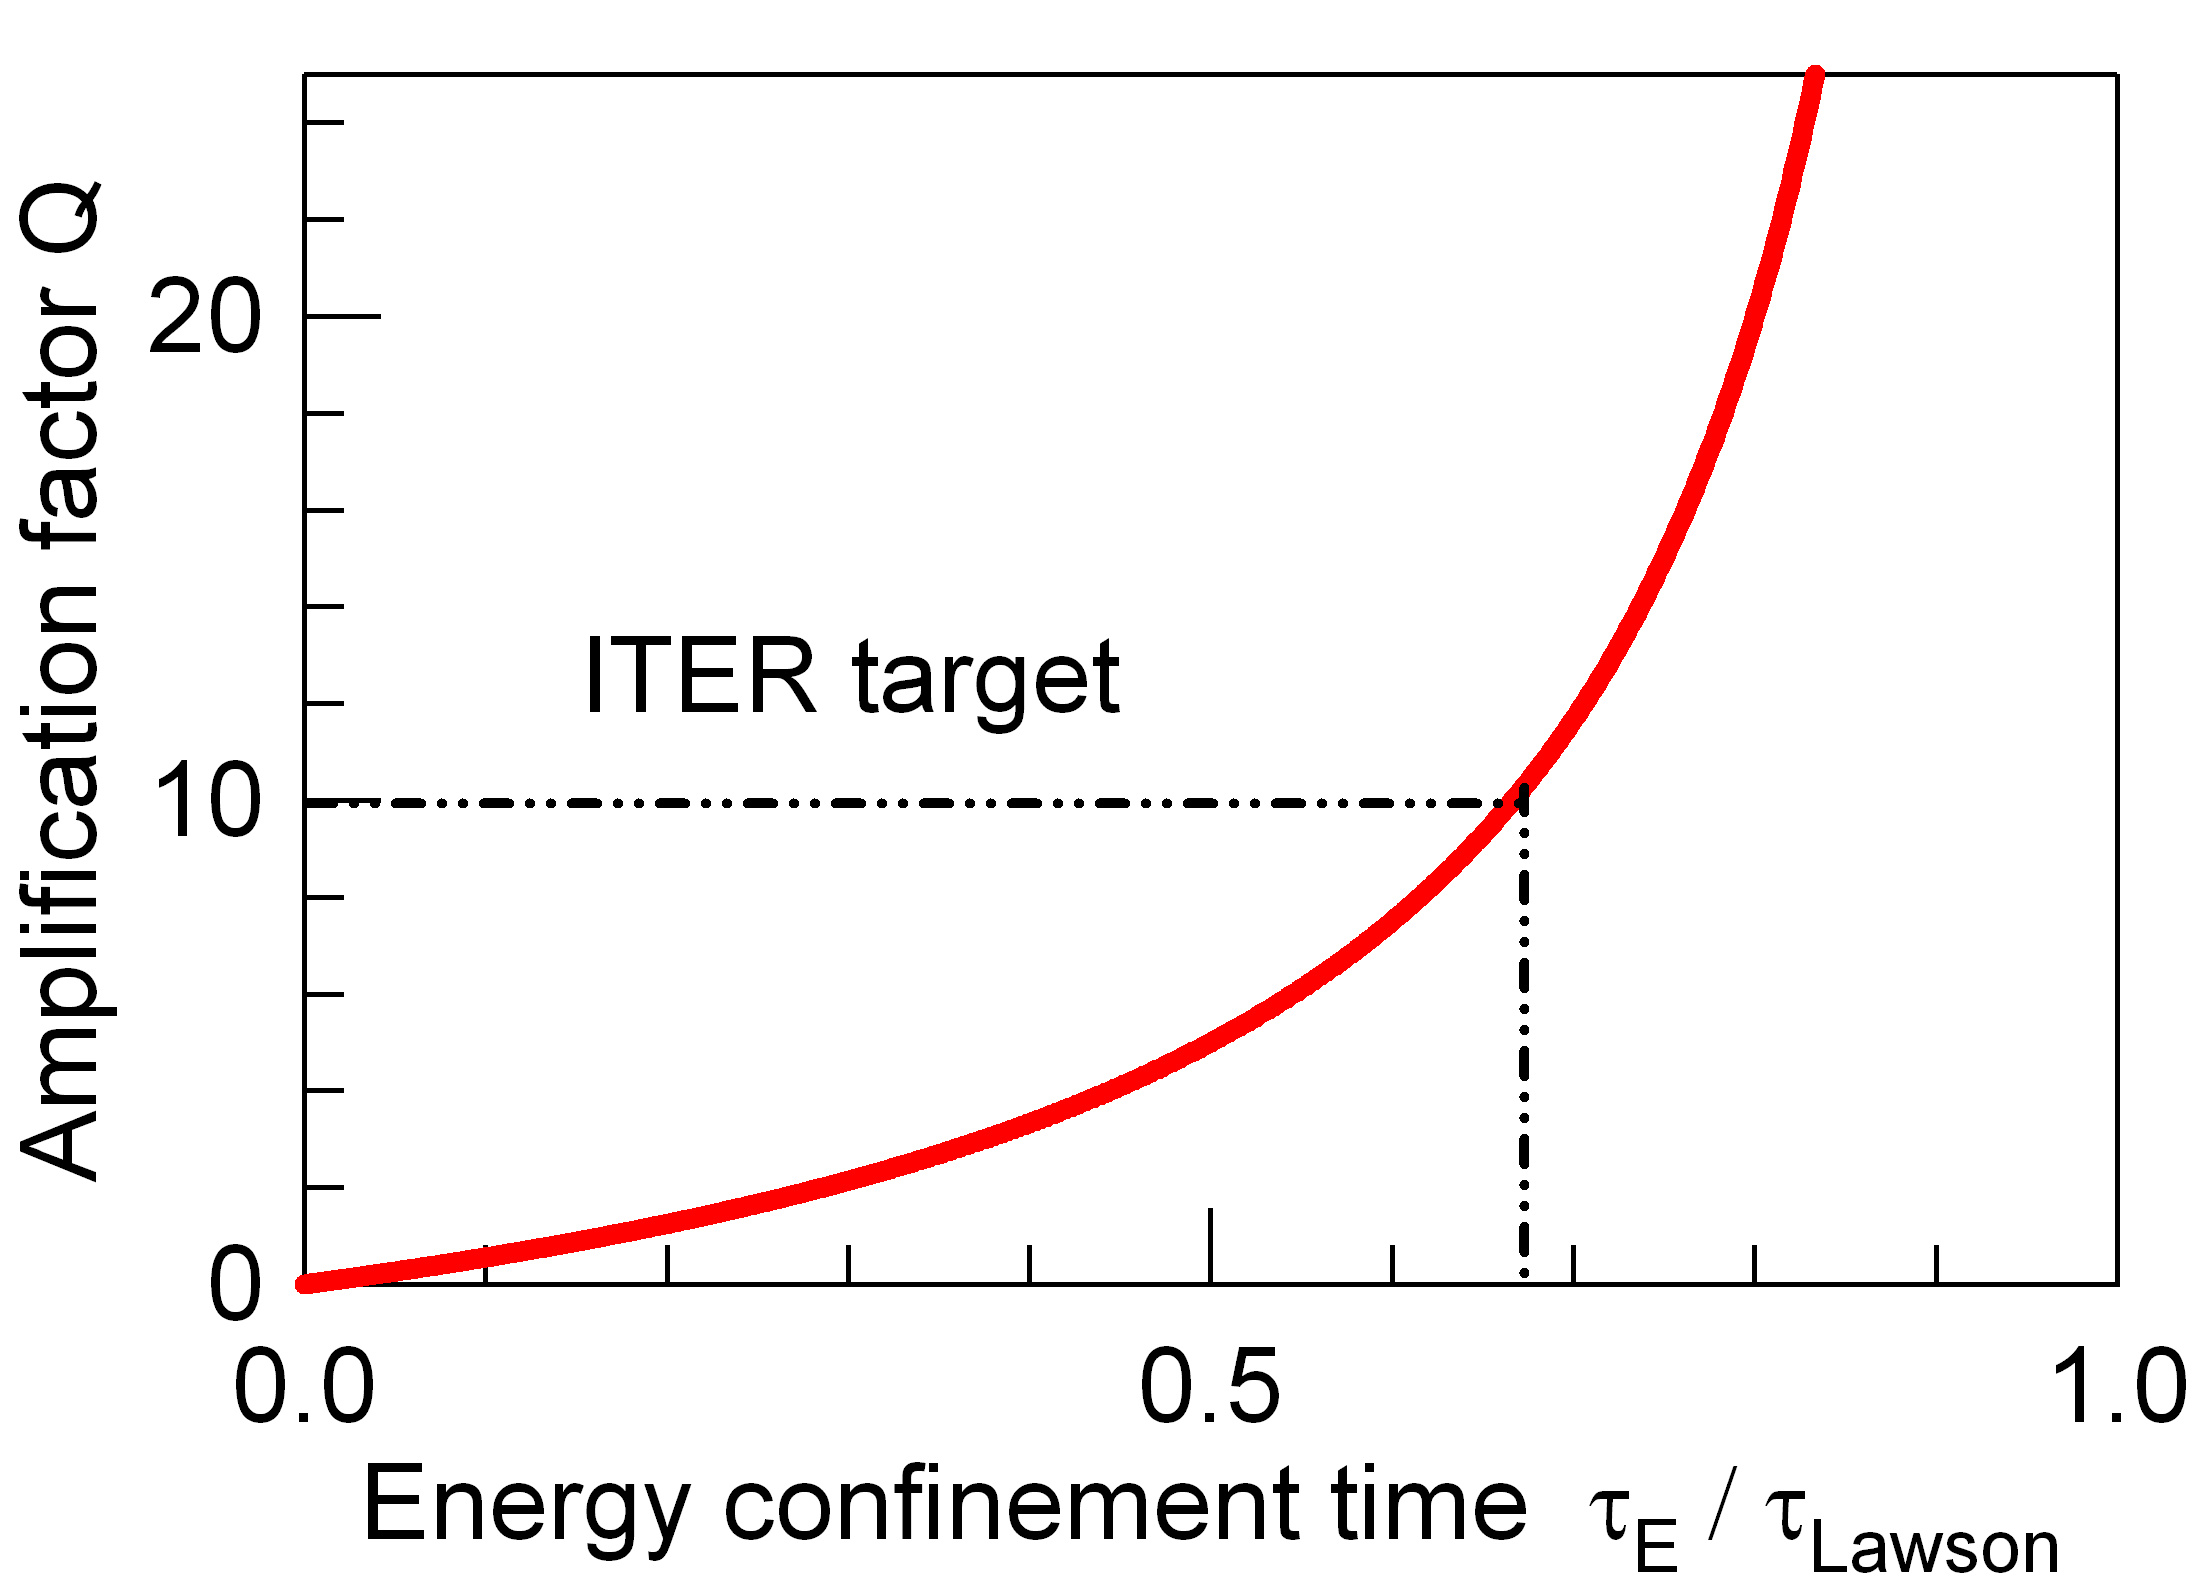
\includegraphics[width=0.65\textwidth]{figures/Graph_Qfactor_tauE.png}
		\caption{Amplification factor $Q$ $versus$ the normalised energy confinement time (see text).}
		\label{fig:Q_tauE}
	\end{center}
\end{figure}


%----------------------------------------------
\subsection{Scaling law of the energy confinement time}
\label{sec:scaling_law}

Experimental results have shown that the energy time in ELMy H-mode tokamak plasmas (referred to as the ITER IPB98(y,2) scaling law \cite[eq.(20)]{ITERphysics_chap2}) is well represented -- the root mean square error is about 15.6\% -- by the following scaling law:
\begin{equation}
  \tau_E = C_{SL} \hat M^{0.19} \kappa^{0.78} \varepsilon^{0.58} 
  \hat n^{0.41} \hat I_p^{0.93} R^{1.97} B^{0.15}  \hat P_{net}^{-0.69}
\end{equation}
with $C_{SL} = 0.0562$.
Here, $\hat I_p$ and $B$ are the plasma current and the toroidal magnetic field at the magnetic axis, respectively, $\hat n$ the line-averaged density, and $\hat M$ is the average ion mass (in Atomic Mass Unit)\footnote{Cf. also \url{http://fusionwiki.ciemat.es/wiki/Scaling_law}.}. 

Introducing the normalised density $n_N = \hat n/\hat n_G$ (eq.\ref{eq:n_nN}) and replacing the current by its expression eq.\ref{eqn:plasma_current}, the scaling law can be recast as follows:
\begin{equation}
  \tau_E = C_{SL} C_n^{0.41} C_I^{1.34} \hat M^{0.19} \kappa^{0.78} \varepsilon^{2.44} q_a^{-1.34}
  n_N^{0.41} R^{2.49} B^{1.49} \hat P_{net}^{-0.69}
\end{equation}

One last step is to replace $\hat P_{net}$ by $\hat P_{loss}$ (eq.\ref{eq:Ploss_betaN}), which is equivalent at equilibrium, and to use the expression of the pressure in terms of $\beta_N$ (eq.\ref{eqn:nT_betaN}) to obtain the following relation:
\begin{equation}
  (\hat n\hat T\tau_E)^{0.31} = C_{SL} C_n^{0.41} C_I^{0.96} C_\beta^{0.38} 
    \hat M^{0.19} \kappa^{0.09} \varepsilon^{0.68} q_a^{-0.96}
    n_N^{0.41} R^{0.42} B^{0.73} \beta_N^{-0.38}
\label{eq:nTtau_betaN}
\end{equation}
The left hand side is fully determined by the value of $Q$, cf. eq.\ref{eq:nTtau_Q}. \\

In turn, eq.\ref{eq:nTtau_betaN} provides an expression of $\beta_N$ as a function of $R$, $B$ and $Q$ at prescribed values of the average ion mass $\hat M$, of geometrical variables ($\kappa$ and $\varepsilon$), of the edge safety factor $q_a$ and of the normalised density $n_N$.
Equation \ref{eq:DT_fusion_power_betaN} is the other independent relation for $\beta_N$, expressed as a function of $R$, $B$ and $P_{DT}$ (again at prescribed $\kappa$, $\varepsilon$ and $q_a$).



